\chapter{Contraction}
\label{ch:design::contraction}

\begin{preamble}
This chapter describes the contraction technique for algorithm design
and applies it to several problems.
%
\end{preamble}


\section{Contraction Technique}
\label{sec:design::contraction}

\begin{gram}
A contraction algorithm has a distinctive anatomy: it has a base case to handle small instances and an inductive step with three
distinct phases: ``contract, ``recur'', and ``expand.''
%
It  involves
solving recursively  smaller instances of the same problem and then expanding the solution for the larger instance.
%
\end{gram}

\begin{definition}[Contraction]
\label{def:design::contraction}

A contraction algorithm for problem $P$ has the following structure.
%

\begin{description}[topsep=1pt,itemsep=1pt]

\item[Base Case:] If the problem instance is sufficiently small, then
  compute and return the solution, possibly using another algorithm.

\item[Inductive Step(s):] If the problem instance is sufficiently large,
  then 


\begin{itemize}
\item 
Apply the following two steps, as many  times as needed.

\begin{enumerate}[topsep=1pt,itemsep=1pt]
\item \defn{Contract:} 
``contract'', i.e., map the instance of the problem $P$ to a smaller
  instance of $P$.

\item \defn{Solve:}
solve the smaller instance recursively.
\end{enumerate}

\item
\defn{Expand} the solutions to smaller instance to solve the original
instance.

\end{itemize}
\end{description}
%

\end{definition}

\begin{remark}
Contraction differs from divide and conquer in that it allows there to
be only one \emph{independent} smaller instance to be recursively
solved.
%
There could be multiple \emph{dependent} smaller instances to be
solved one after another (sequentially).
\end{remark}

\begin{gram}[Properties of Contraction]

Contraction algorithms have several important properties.  

\begin{itemize}
\item Due to their inductive structure, we can establish the
  correctness of a contraction algorithm using principles of
  induction: we first prove correctness for the base case, and then
  prove the general (inductive) case by using strong induction, which
  allows us to assume that the recursive call is correct.

\item 
The work and span of a contraction algorithm can be expressed as a
mathematical recurrence that reflects the structure of the algorithm
itself. Such recurrences can then unually be solved using
well-understood techniques, and without significant difficulty.

%
\item 
Contraction algorithms can be work efficient, if they can reduce the
problem size geometrically (by a constant factor greater than $1$) at
each contraction step, and if the contraction and the expansions steps
are efficient.
%

\item Contraction algorithms can have a low span (high parallelism),
  if size of the problem instance decreases geometrically, and if
  contraction and expansion steps have low spans.

\end{itemize}


%
\end{gram}


\begin{example}[Maximal Element]
We can find the maximal element in a sequence $a$ using contraction as
follows.
%
If the sequence has only one element, we return that element,
%
otherwise,
%
we can map the sequence $a$ into a sequence $b$ which is half the
length by comparing the elements of $a$ at consecutive even-odd
positions and writing the larger into $b$.
%
We then find the largest in $b$ and return this as the result.

For example, we map the sequence
%
$\cseq{1,2,4,3,6,5}$ 
%
to 
%
$\cseq{2,4,6}$.
% 
The largest element of this sequence, $6$ is then the largest element
in the input sequence.
%

%
For a sequence of length $n$, we can write the work and span for this
algorithm as recurrences as follows
\[
W(n) = \left\{
\begin{array}{lll}
\Theta(1) & \mbox{if} & n \le 1
\\
W(n/2) + \Theta(n) &  \mbox{otherwise}
\end{array}
\right.
\]
%
\[
S(n) = \left\{
\begin{array}{lll}
\Theta(1) & \mbox{if} & n \le 1
\\
S(n/2) + \Theta(1) &  \mbox{otherwise}.
\end{array}
\right.
\]
%
Using the techniques discussed at the end of this chapter, we can solve
the recurrences to obtain $W(n) = \Theta(n)$ and $S(n) =
\Theta(\lg{n})$.
\end{example}

\section{Reduce with Contraction}
\label{sec:design::contraction::reduce}

\begin{gram}
The~\defn{reduce} primitive performs a computation that involves
applying an associative binary operation $op$ to the elements of a
sequence to obtain (reduce the sequence to) a final value.
%
For example, reducing the sequence $\cseq{0,1,2,3,4}$ with the $+$
operation gives us $0 + 1 + 2 + 3 + 4 = 10$.
%
Recall that the type signature for~$\cdvar{reduce}$ is as follows.
%
\[
\cdvar{reduce}~(f: \alpha * \alpha \ra \alpha)~(\cdvar{id}: \alpha)~(a: \sseq{\alpha}): \alpha,
\]
where $f$ is a binary function, $a$ is the sequence, and $\cdvar{id}$
is the left identity for $f$.
%

%In section \ref{seq}
Even though we can define $\cdvar{reduce}$ broadly for both associative
and non-associative functions, in this section, we assume that the
function~$f$ is associative.

\end{gram}

\begin{gram}
Generalizing the algorithm for computing the maximal element leads us
to an implementation of an important parallelism primitive called $\cdvar{reduce}$.
%
The crux in using the contraction technique is to design an algorithm
for reducing an instance of the problem to a geometrically smaller
instance by performing a parallel contraction step.
%
To see how this can be done, consider instead applying the
function~$f$ to consecutive pairs of the input.
%

For example if we wish to compute the sum of the input sequence 
\[
\cseq{ 2,1,3,2,2,5,4,1}
\]
by using the addition function, we can contract the sequence to
\[
\cseq{ 3, 5, 7, 5 }.
\]
%
Note that the contraction step can be performed in parallel, because
each pair can be considered independently in parallel.

By using this contraction step, we have reduced the input size by a
factor of two.
%
We next solve the resulting problem by invoking the same algorithm and
apply expansion to construct the final result.
%
We note now that by solving the smaller problem, we obtain a solution
to the original problem, because the sum of the sequence remains the
same as that of the original.  Thus, the expansion step requires no
additional work.
%
\end{gram}

\begin{algorithm}[Reduce with Contraction]
\label{alg:design::contraction::reduce}
An algorithm for $\cdvar{reduce}$ using contraction is shown below; for
simplicity, we assume that the input size is a power of two.
%

\[
\begin{array}{l}
\cd{(* Assumption:}~|a|~\cd{is a power of 2 *)}
\\
\cdvar{reduceContract}~f~\cdvar{id}~a =
\\ 
~~~~\cd{if}~|a| = 1~\cd{then}
\\
~~~~~~~~a[0]
\\
~~~~\cd{else}
\\ 
~~~~~~~~\cd{let}
\\
~~~~~~~~~~~~b = \cseq{f(a[2i],a[2i+1]) : 0 \le i < \lfloor |a|/2
  \rfloor}
\\ 
~~~~~~~~\cd{in}
\\
~~~~~~~~~~~~\cdvar{reduceContract}~f~\cdvar{id}~b
\\
~~~~~~~~\cd{end}
\end{array}
\]
\end{algorithm}
%

\begin{gram}[Cost of Reduce with Contraction]
Assuming that the function being reduced over performs constant work, 
parallel tabulate in the contraction step requires linear work, 
we can thus write the work of this algorithm as 
\[
W(n) = W(n/2) + n.
\]
This recurrence solves to $O(n)$.
%


Assuming that the function being reduced over performs constant span, 
parallel tabulate in the contraction step requires constant span;
we can thus write the work of this algorithm as
%
\[
S(n) = S(n/2) + 1.
\]
This recurrence solves to $O(\log{n})$.
\end{gram}

\section{Scan with Contraction}
\label{sec:design::contraction::scan}

\begin{gram}
We describe how to implement the $\cdvar{scan}$ sequence primitive
efficiently by using contraction.
%
Recall that 
the $\cdvar{scan}$ function has the type signature
\[
\cdvar{scan}~(f: \alpha * \alpha \ra \alpha)~(\cdvar{id}: \alpha)~(a: \sseq{\alpha})~:~(\sseq{\alpha} * \alpha)
\]
where $f$ is an associative function, $a$ is a sequence, and
$\cdvar{id}$ is the identity element of $f$.
%
When evaluated with a function and a sequence, $\cdvar{scan}$ can be
viewed as applying a reduction to every prefix of the sequence and
returning the results of such reductions as a sequence.
%
\end{gram}

\begin{example}
Applying $\cdvar{scan}~`+`$, i.e., ``plus scan'' on the sequence
$\cseq{2,1,3,2,2,5,4,1}$ returns
\[
\left(\cseq{0, 2, 3, 6, 8, 10, 15, 19}, 20\right).
\]
We will use this as a running example.
\end{example}

\begin{gram}
Based on its specification, a direct algorithm for $\cdvar{scan}$ is to
apply a reduce to all prefixes of the input sequence.  
%
Unfortunately, this easily requires quadratic work in the size of the
input sequence.
%

We can see that this algorithm is inefficient by noting that it
performs lots of redundant computations.  In fact, two consecutive
prefixes overlap significantly but the algorithm does not take
advantage of such overlaps at all, computing the result for each
overlap independently. 
%

By taking advantage of the fact that any two consecutive prefixes
differ by just one element, it is not difficult to give a linear work
algorithm (modulo the cost of the application of the argument
function) by using iteration.  

Such an algorithm may be expressed as
follows
\[
\cdvar{scan}~f~\cdvar{id}~{a} = h \left( \cdvar{iterate}~g~(\cseq{},id)~a \right), 
\]
where
\[ 
g((b, y), x) = ((\cdvar{append} \cseq{y} b),~f(y,x))~
\]
\\
and 
\\
\[
h (b,y) = ((\cdvar{reverse}~b), y)
\]
where $\cdvar{reverse}$ reverses a sequence.
%

This algorithm is correct but it almost entirely sequential, leaving
no room for parallelism.

\end{gram}


\begin{gram}[Scan via Contraction, the Intuition]

Because $\cdvar{scan}$ has to compute some value for each
prefix of the given sequence, it may appear to be inherently sequential.  
%
We might be inclined to believe that any efficient algorithms will
have to keep a cumulative ``sum,'' computing each output value by
relying on the ``sum'' of the all values before it.  
%

We will now see that we can implement $\cdvar{scan}$ efficiently using contraction.  To this
end, we need to reduce a given problem instance to a geometrically
smaller instance by applying a contraction step.
%
As a starting point, let's apply the same idea as we used for
implementing 
%
\href{alg:design::contraction::reduce}{reduce with contraction}.
%

Applying the contraction step from the $\cdvar{reduce}$ algorithm
described above, we would reduce the input sequence
\[
\cseq{2,1,3,2,2,5,4,1}
\]
to the sequence
\[
\cseq{3,5,7,5},
\]
which if recursively used as input would give us the result
\[
(\cseq{ 0, 3, 8, 15 }, 20).
\]
Notice that in this sequence, the elements in even numbered positions are consistent with the desired result:
\[
(\cseq{0, 2, 3, 6, 8, 10, 15, 19}, 20).
\]

Half of the elements are correct because the
contraction step, which pairs up the elements and reduces them, does
not affect, by associativity of the function being used, the result at
a position that do not fall in between a pair.  
%

To compute the missing element of the result, we will use an expansion
step and compute each missing elements by applying
the function element-wise to the corresponding elements in the input and the results of the recursive call to $\cdvar{scan}.$
%
The drawing below illustrates this expansion step.
\begin{center}
  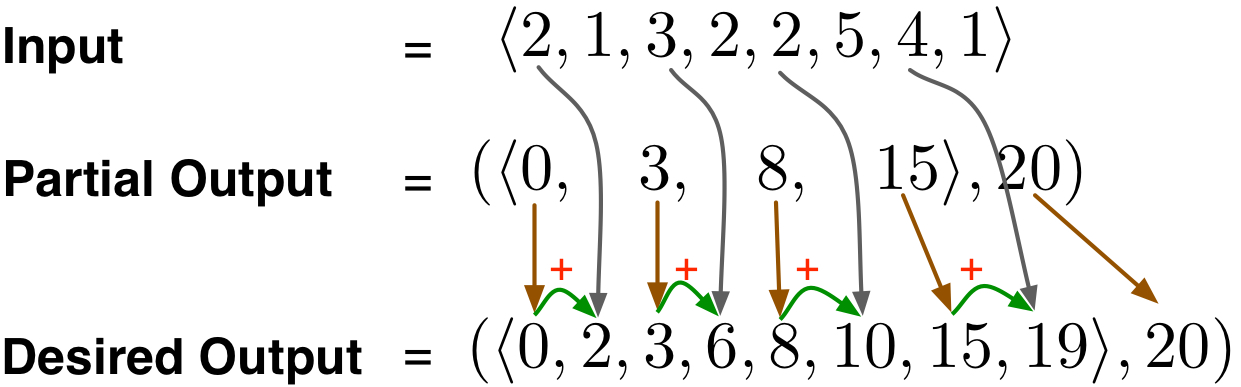
\includegraphics[width=4in]{./design/media-contraction/prefix-eval.jpg}
\end{center}
\end{gram}


\begin{algorithm}[Scan Using Contraction, for Powers of 2]
\label{alg:design::contraction::scan}

Based on the intuitive description above, we can write the pseudo-code
for $\cdvar{scan}$ as  follows.
%
For simplicity, we assume that $n$ is a power of two.
%

\[
\begin{array}{l}
\cd{(* Assumption:}~|a|~\cd{is a power of two. *)}
\\
\cdvar{scan}~f~\cdvar{id}~a =
\\
~~~~\cd{if}~|a| = 0~\cd{then} 
\\
~~~~\left(\cseq{}, id\right)
\\
~~~~\cd{else if}~|a| = 1 ~\cd{then}
\\
~~~~~~~~\left( \cseq{id}, a[0] \right)
\\
~~~~\cd{else}
\\ 
~~~~~~~~\cd{let}
\\
~~~~~~~~~~~~a' = \cseq{ f(a[2i],a[2i+1]) : 0 \leq i < n/2}
\\
~~~~~~~~~~~~(r,t) = \cdvar{scan}~f~\cdvar{id}~ a'
\\
~~~~~~~~\cd{in}
\\ 
~~~~~~~~~~~~(\cseq{ p_i : 0 \leq i < n }, t),~\com{where}~p_i = 
%
\begin{cases}
     r[i/2]  & \cd{even}(i) \\
     f(r[i/2], a[i-1]) & \cd{otherwise}
\end{cases}
%
\\
~~~~~~~~\cd{end}
\end{array}
\]
\end{algorithm}


\begin{gram}[Cost of Scan with Contraction]
Let's assume for simplicity that the function being applied has
constant work and constant span. We can write out the work and span
for the algorithm as a recursive relation as 
\begin{align*}
W(n) &= W(n/2) + n,~\mbox{and}
\\
S(n) &= S(n/2) + 1,
\end{align*}
because 1) the contraction step which tabulates the smaller instance
of the problem performs linear work in constant span, and 2) the
expansion step that constructs the output by tabulating based on the
result of the recursive call also performs linear work in constant
span.

These recursive relations should look familiar.  They are the same as
those that we ended up with when we analyzed the work and span of our
contraction-based implementation of $\cdvar{reduce}$ and  yield 
\begin{align*}
W(n) &= O(n)
\\
S(n) &=  O(\log{n}).
\end{align*}
\end{gram}

%% \begin{checkpoint}

%% \begin{questionfr}[Ranking sequences]
%% \points 10
%% \prompt

%%   Given a sequence of $n$ natural numbers and and a rank $r < n$, you
%%   want to find the element of the sequence with the given rank. For
%%   example if the input is $\cseq{1,3,2,4}$ and you are asked to find
%%   the element with rank $0$ then the answer is $1$ because $1$ is the
%%   element with rank $0$, i.e., the smallest element.

%% \begin{itemize}
%% \item Using the contraction technique, design an algorithm for finding
%%   the element of the sequence with a given rank.

%% \item Analyze the worst-case work and span of your algorithm.

%% \item Analyze the best-case work and span of your algorithm.
%% \end{itemize}
%% \answer
%% \end{questionfr}

%% \end{checkpoint}

